% Gemini theme
% https://github.com/anishathalye/gemini

\documentclass[final]{beamer}

% ====================
% Packages
% ====================

\usepackage[size=custom,width=36,height=48,scale=0.4]{beamerposter}
\usetheme{gemini}
\usecolortheme{mit}
\usepackage{graphicx}
\usepackage{booktabs}
\usepackage{tikz}
\usepackage{pgfplots}
\pgfplotsset{compat=1.18}

%% LuaLatex with Libertine font
\usepackage[libertine]{newtxmath}
\usepackage[stretch=10,shrink=10]{microtype}
\setmainfont{Linux Libertine O}
  [Ligatures={Common,Rare,Historic}, Numbers=OldStyle]

% ====================
% Lengths
% ====================

% If you have N columns, choose \sepwidth and \colwidth such that
% (N+1)*\sepwidth + N*\colwidth = \paperwidth
\newlength{\sepwidth}
\newlength{\colwidth}
\setlength{\sepwidth}{0.025\paperwidth}
\setlength{\colwidth}{0.42\paperwidth}

\newcommand{\separatorcolumn}{\begin{column}{\sepwidth}\end{column}}

% Fix Beamer bibtex styling
\setbeamertemplate{bibliography entry article}{}
\setbeamertemplate{bibliography entry title}{}
\setbeamertemplate{bibliography entry location}{}
\setbeamertemplate{bibliography entry note}{}

% ====================
% Title
% ====================

\title{Continuous Ground-based Observation of Low-altitude Cloud Properties at the Zeppelin Observatory}

\author{GUNHO (LOREN) OH \inst{1} \and SANGJONG PARK \inst{1}}

\institute[shortinst]{\inst{1} Korea Polar Research Institute (KOPRI)}

% ====================
% Footer (optional)
% ====================

\footercontent{
Korea Polar Research Institute (KOPRI), Incheon, Korea \hfill \null
}
% (can be left out to remove footer)

% ====================
% Logo (optional)
% ====================

% use this to include logos on the left and/or right side of the header:
% \logoright{\includegraphics[height=7cm]{logo1.pdf}}
% \logoleft{\includegraphics[height=7cm]{logo2.pdf}}

% ====================
% Body
% ====================

\begin{document}

\begin{frame}[t]
\begin{columns}[t]
\separatorcolumn

\begin{column}{\colwidth}

  \begin{alertblock}{Introduction}
    The largest source of uncertainty in estimating the radiative response to a warming climate in global climate models comes from the representation of clouds, which modulate the radiative transfer through the atmosphere and drive a number of feedback processes. The uncertainty in our prediction of the Arctic climate is further exacerbated by Arctic amplification processes. Despite their importance, however, our understanding of dynamic and thermodynamic properties of clouds is still far from complete. This is largely due to the difficulties involved in making detailed observations of the properties of the Arctic clouds. To this end, continuous in-situ measurements of liquid droplets were made at the Zeppelin Observatory, Svalbard, using a cloud particle spectrometre called the Cloud Droplet Probe. Post-processed time-series of cloud liquid water concentration (LWC) is presented and examined against existing in-situ observations of cloud particle size distributions; the results show that these measurements provide a detailed look at the properties of low-altitude cloud properties, which can be used to help take a closer look at convective activities in the Arctic atmosphere.
  \end{alertblock}

  \begin{block}{Methods}
    The cloud particle spectrometer (CDP2) has been measuring some of the key thermodynamic and microphysical properties of low-altitude clouds at the Zeppelin Observatory, near Ny-\r{A}lesund, Svalbard, since 2017. The following figure shows a time-series of the monthly mean values of cloud liquid water concentration (LWC).

    \begin{figure}
        \centering
        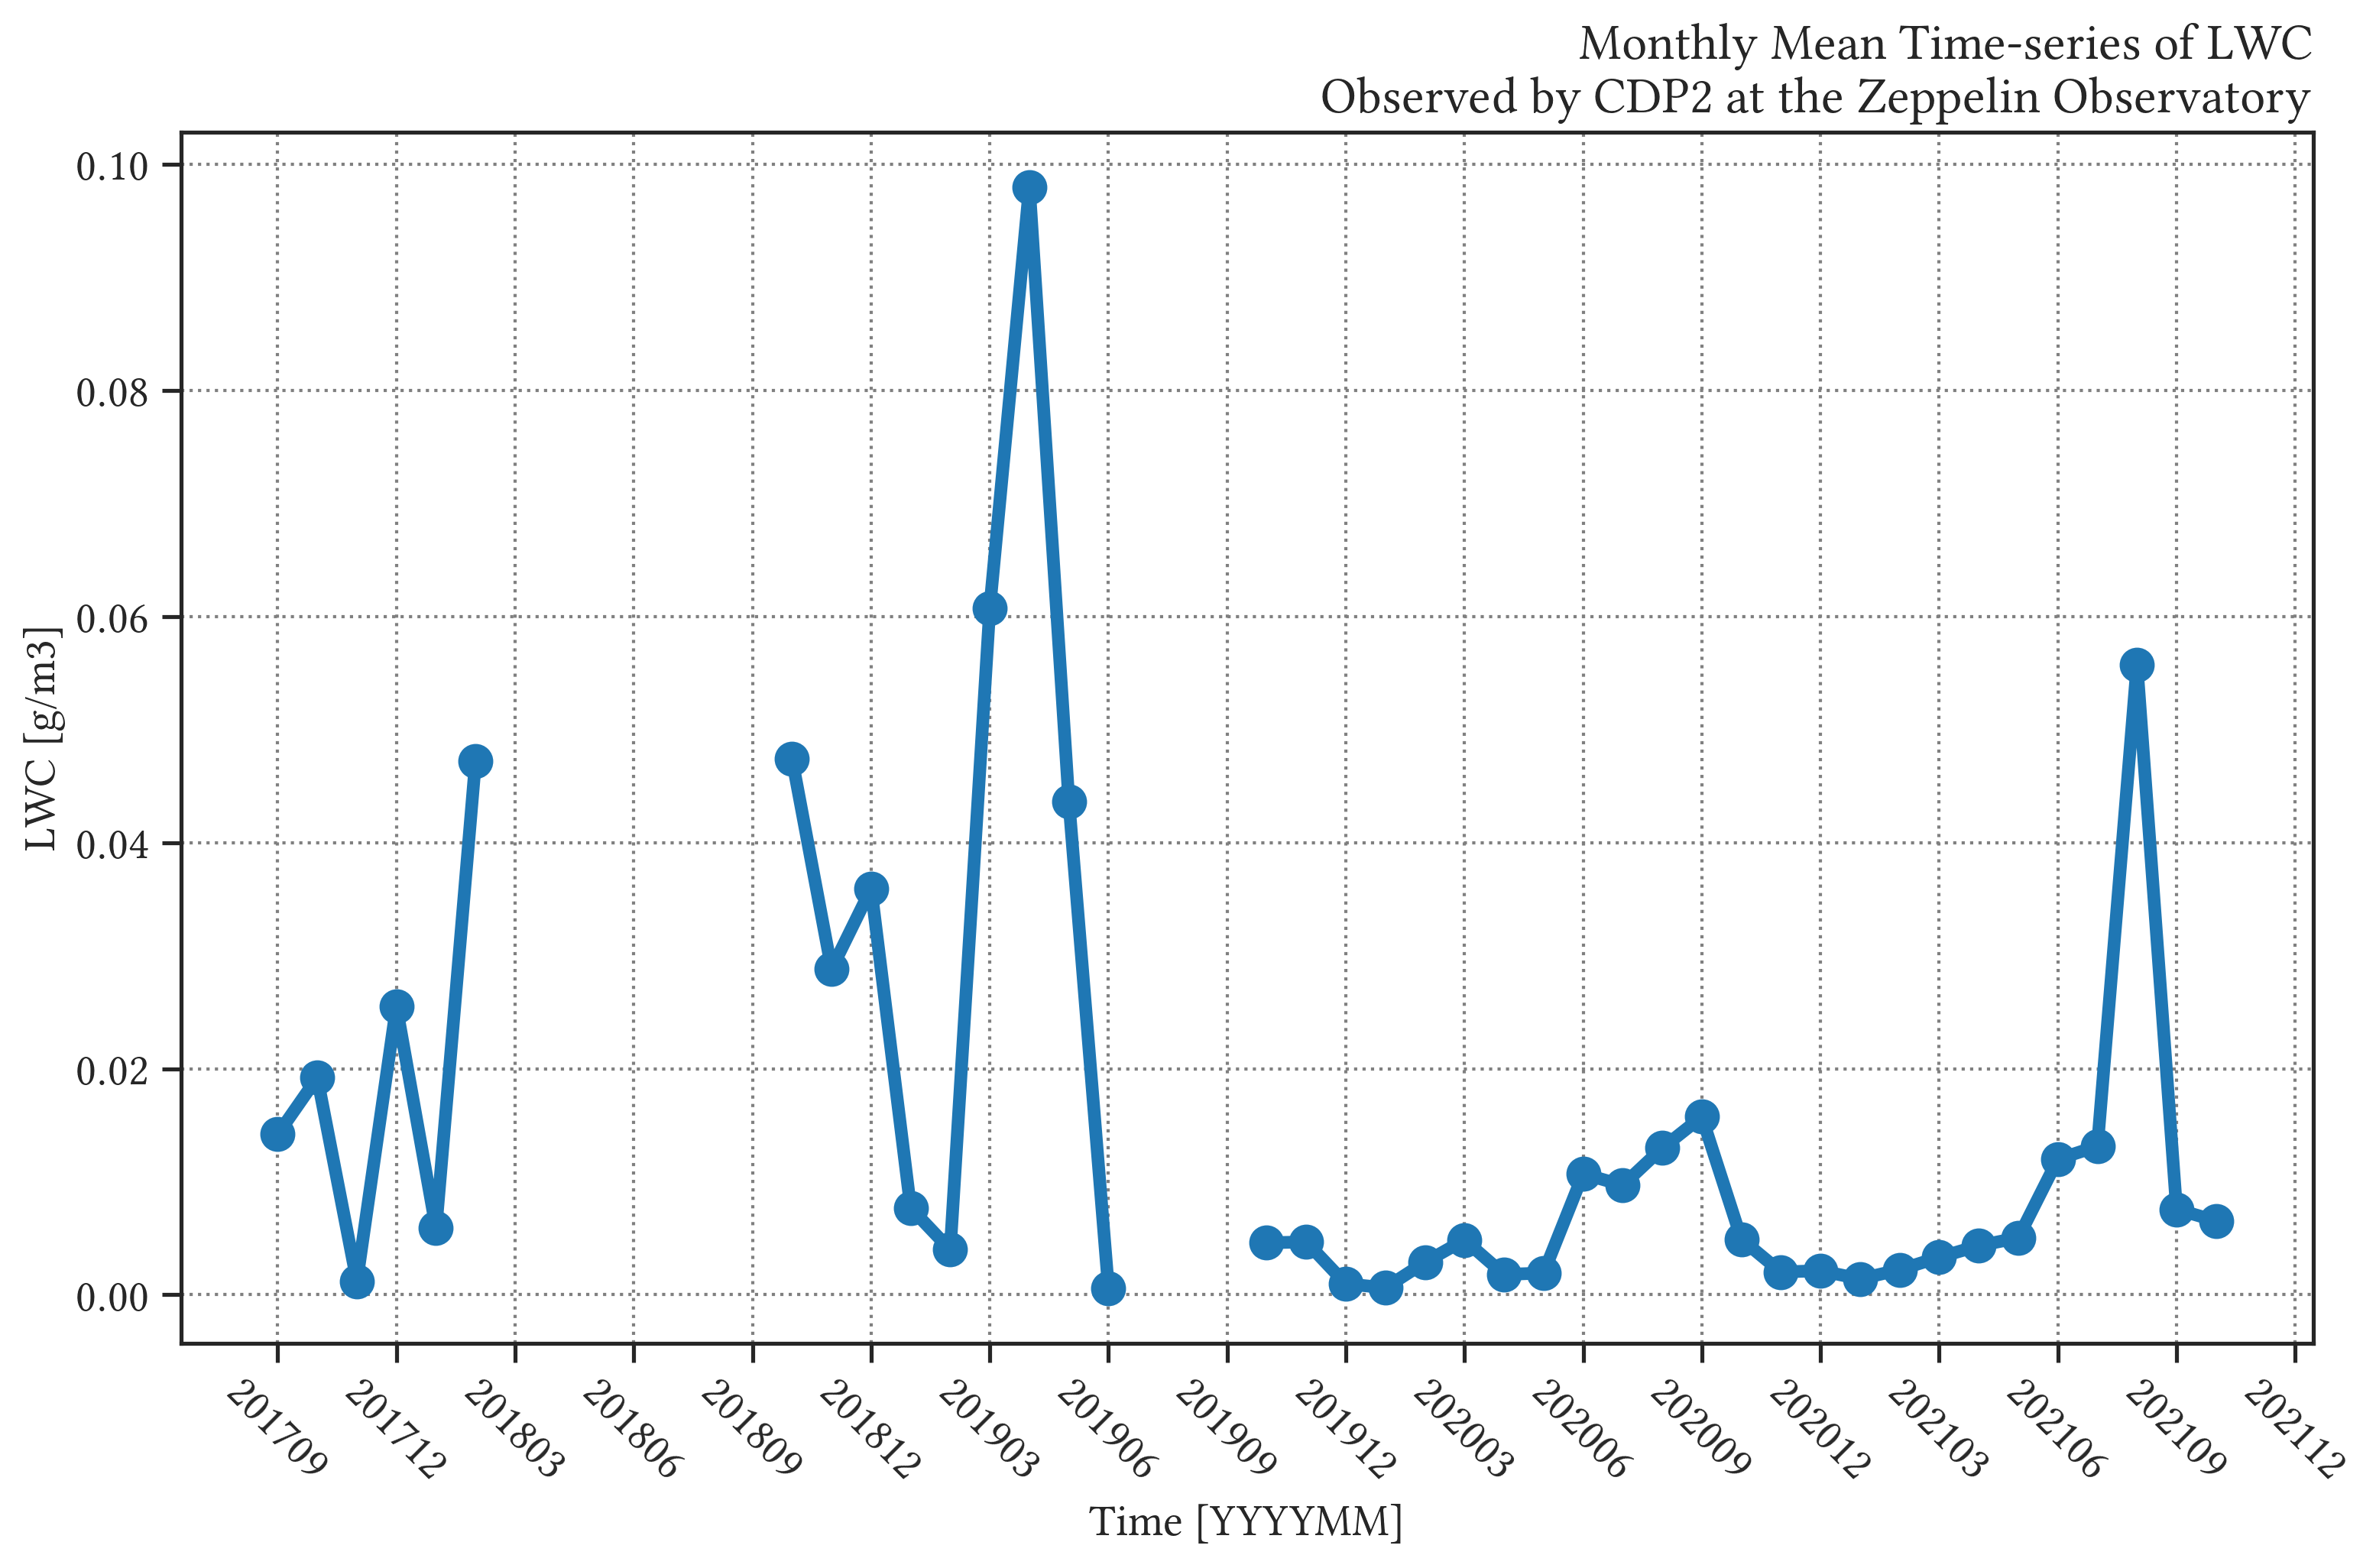
\includegraphics[width=\colwidth]{img/monthly.png}
        \caption{ Monthly average values of liquid water content (LWC) [g/m$^3$], observed by the cloud particle spectrometer (CDP2). Each measurement point represents an average of all daily LWC values for the corresponding month. Daily values of LWC below 1e-3 g/m$^3$ are excluded from calculations to reduce observational noise. }
        \label{fig:01}
    \end{figure}

    CDP2 measures a number of thermodynamic and microphysical properties of low-altitude clouds, such as cloud liquid water concentration (LWC), number concentration (NC) and particle size distribution every 10 seconds. Here, we focus on the time-series evolution of LWC observed on November 8th, 2019, for a qualitative comparison between the measurements from CDP2 and those from an existing in-situ observation (FM120 \cite{karl2020ro,koik2019ye}) at the Zeppelin Observatory.

    The high-resolution time-series of LWC obtained from CDP2 needs to be further processed for a statistical analysis. For this purpose, we employed Gaussian Process Regression (GP) method \cite{rasm2006ga} to identify the underlying behaviour from the noisy time-series. Figure \ref{fig:02} below shows the result of applying the GP model, based on a Square-Exponential (SE) kernel, to retrieve a smooth time-series from the 10-second observation with noise. The SE kernel is governed by a time-scale parameter $\lambda$, which is used to represent our prior belief that the true properties of the cloud particles vary relatively slowly in time.

    \begin{figure}
        \centering
        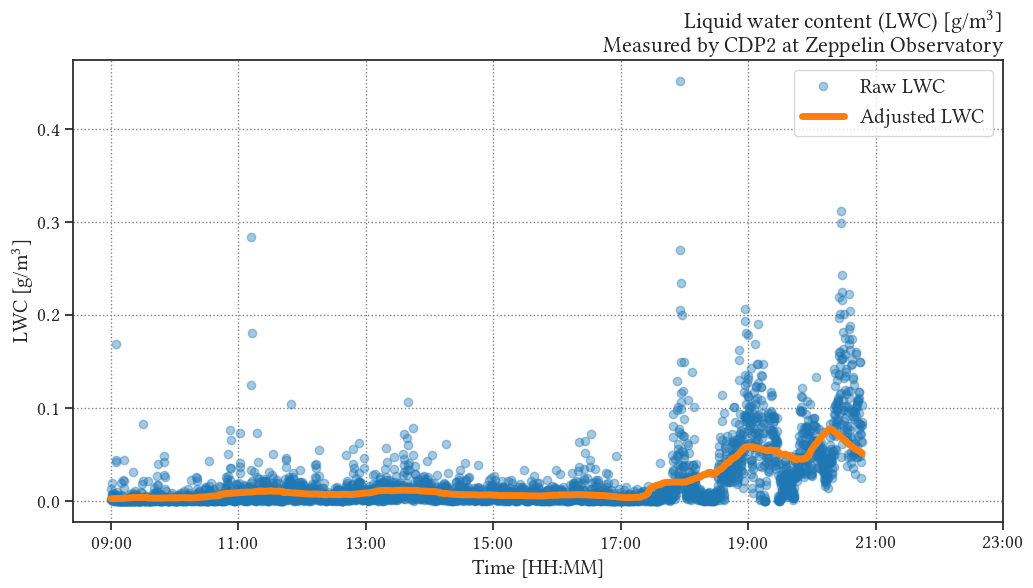
\includegraphics[width=\colwidth]{img/lwc_raw.png}
        \caption{ The time-series of cloud liquid water content (LWC) [g/m$^3$] measured by CDP2 on November 8th, 2019, at the Zeppelin Observatory near Ny-\r{A}lesund, Svalbard. Blue dots show raw observation points from CDP2, and the orange curve represents the smooth distribution modelled by the GP method. }
        \label{fig:02}
    \end{figure}
  \end{block}

\end{column}

\separatorcolumn

\begin{column}{\colwidth}

  \begin{block}{Results}
    Figures \ref{fig:03} and \ref{fig:04} show the observed time-series of LWC in [g/m$^3$], based on the GP method. The two probes correspond well to each other, especially at the peak of the distribution. However, FM120 tends to generally underestimate the values of LWC compared to those from CDP2, although the difference between the two measurements are small in scale.

    The GP model is particularly useful in making a statistical comparison from the two time-series. Since the measurements have been taken at different times, we can produce the GP posterior distribution which can be sampled exactly at same intervals. The orange points in Figures \ref{fig:03} and \ref{fig:04} correspond to samples taken at the same sampling points for the two probes, which allows us to take a direct comparison between the two measurements.

    \begin{figure}
        \centering
        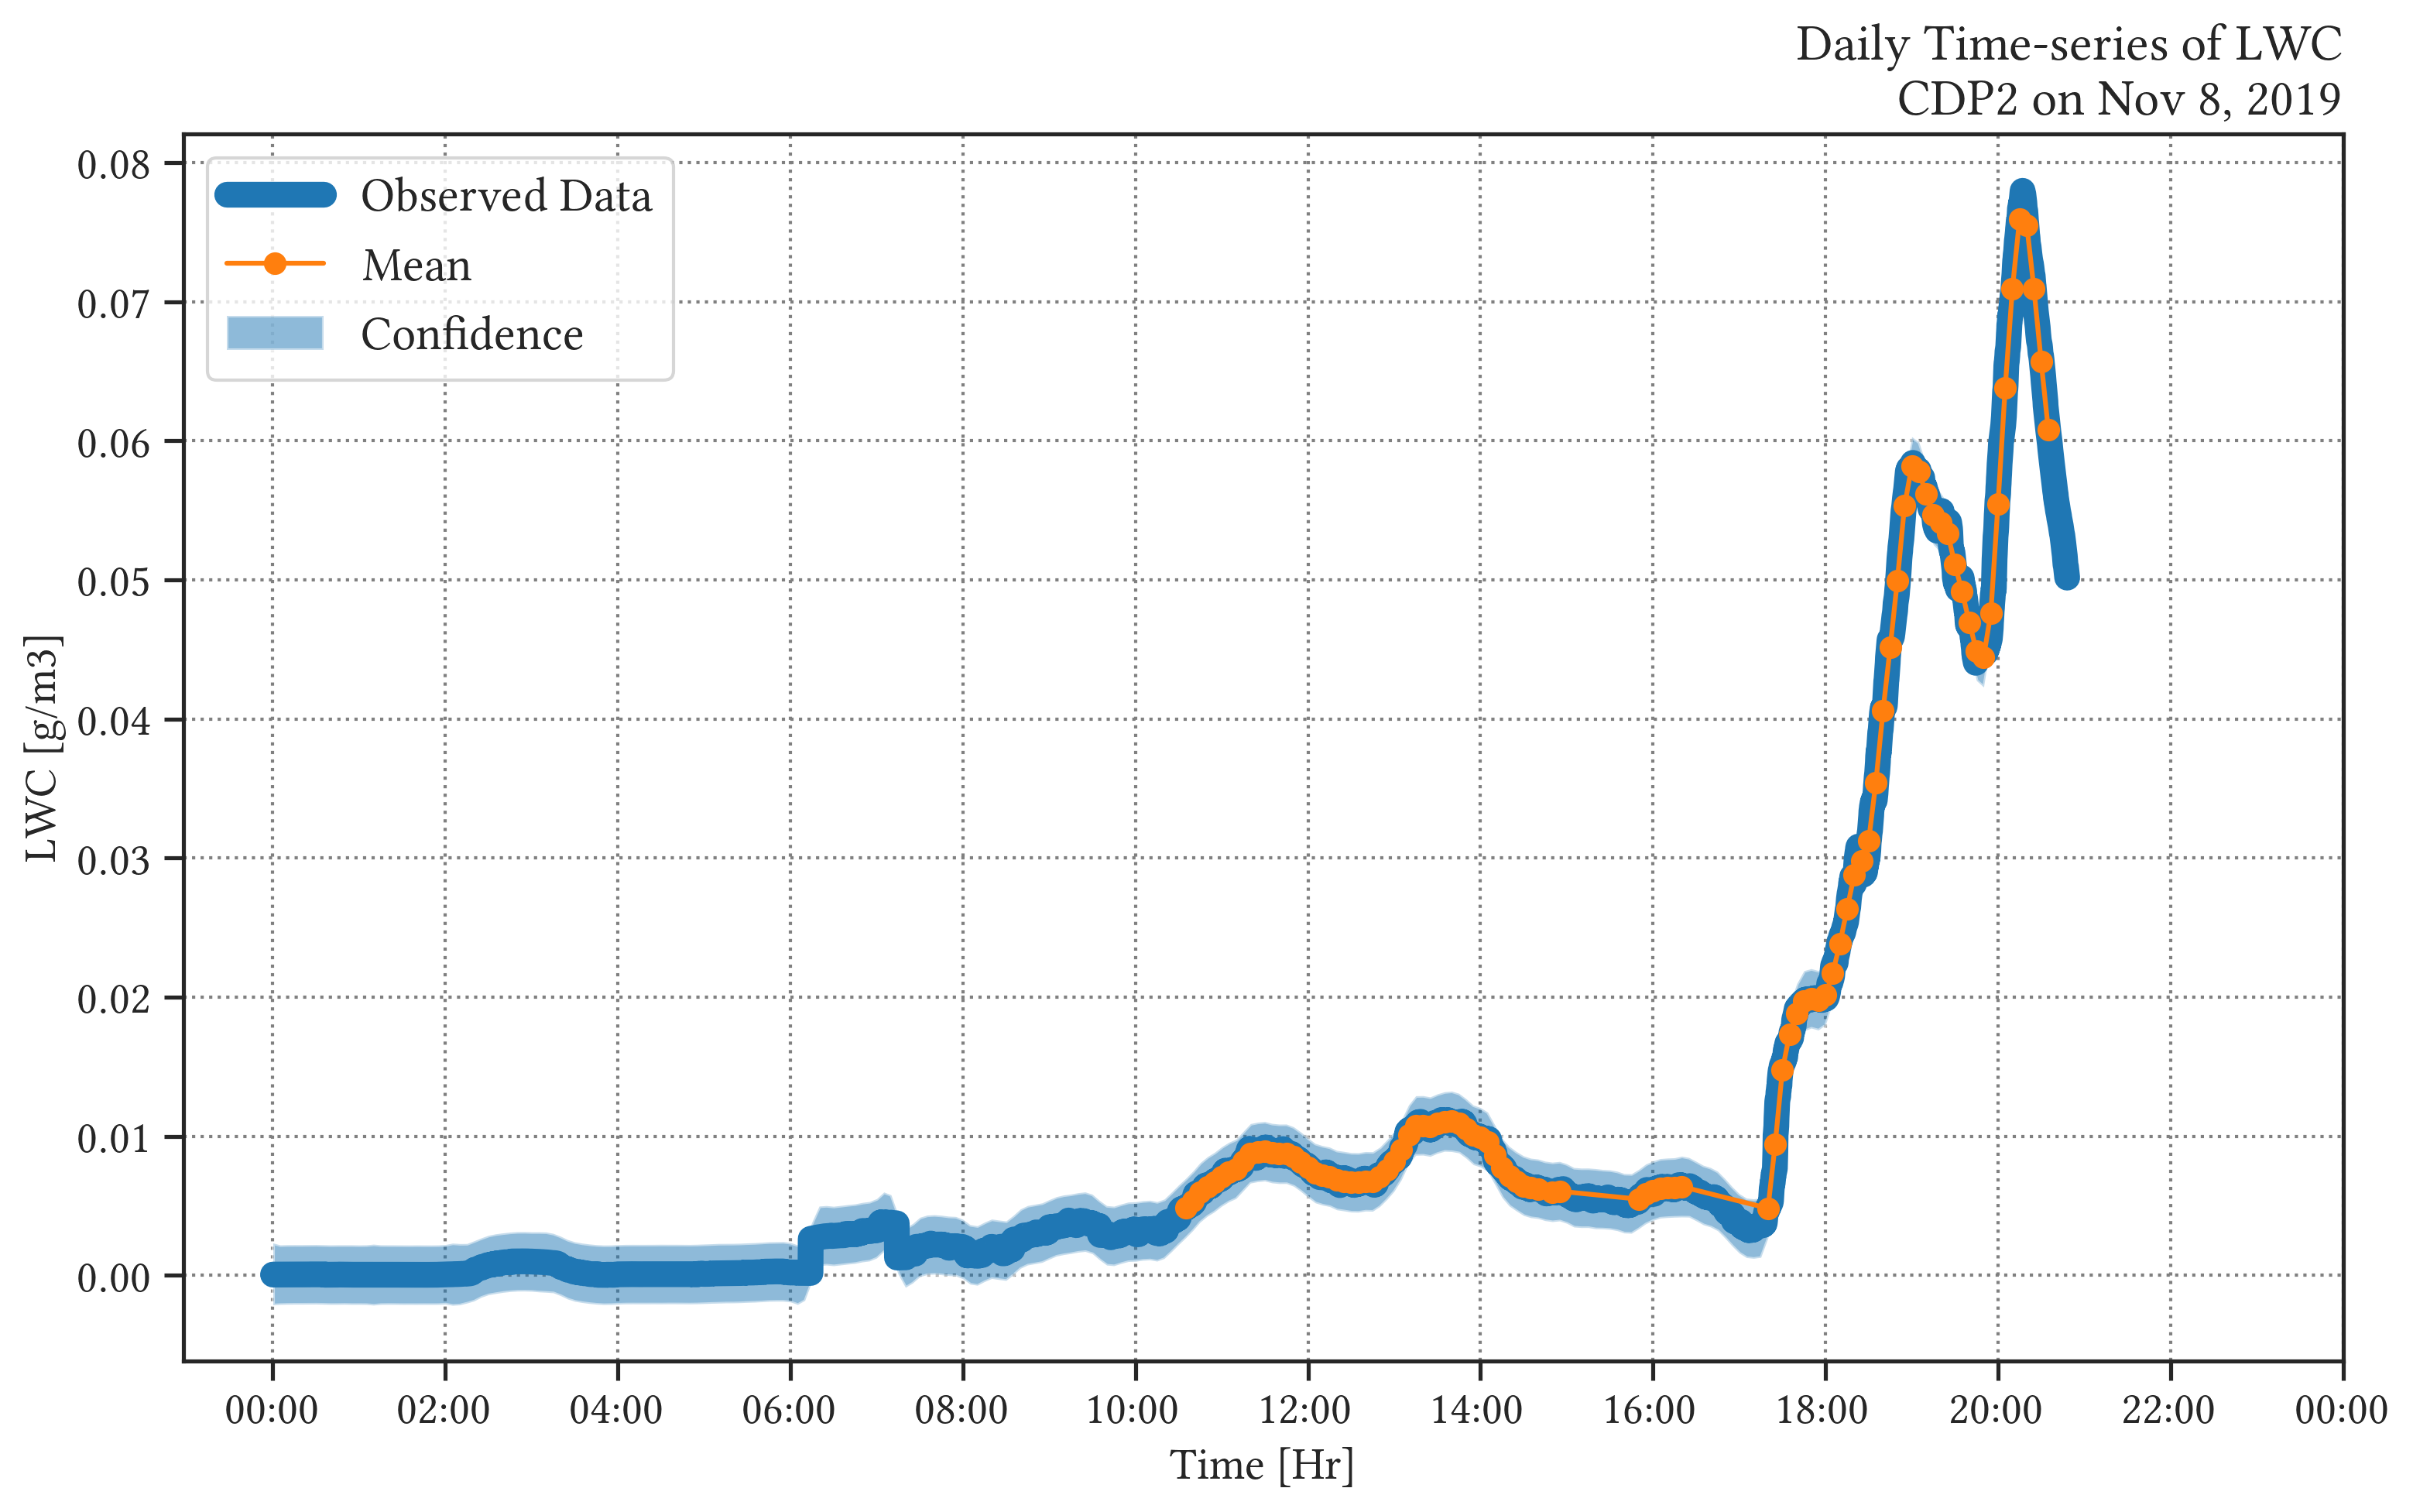
\includegraphics[width=\colwidth]{img/lwc_cdp.png}
        \caption{ The time-series of cloud liquid water content (LWC) [g/m$^3$] measured by CDP2 on November 8th, 2019, at the Zeppelin Observatory near Ny-\r{A}lesund, Svalbard. Blue dots represent smooth GP posterior (\emph{cf.} Figure \ref{fig:02}), and the orange dots have been sampled from the posterior at a 10-minute interval. The shaded region denotes the 95\% confidence region for the GP posterior distribution. }
        \label{fig:03}
    \end{figure}

    \begin{figure}
        \centering
        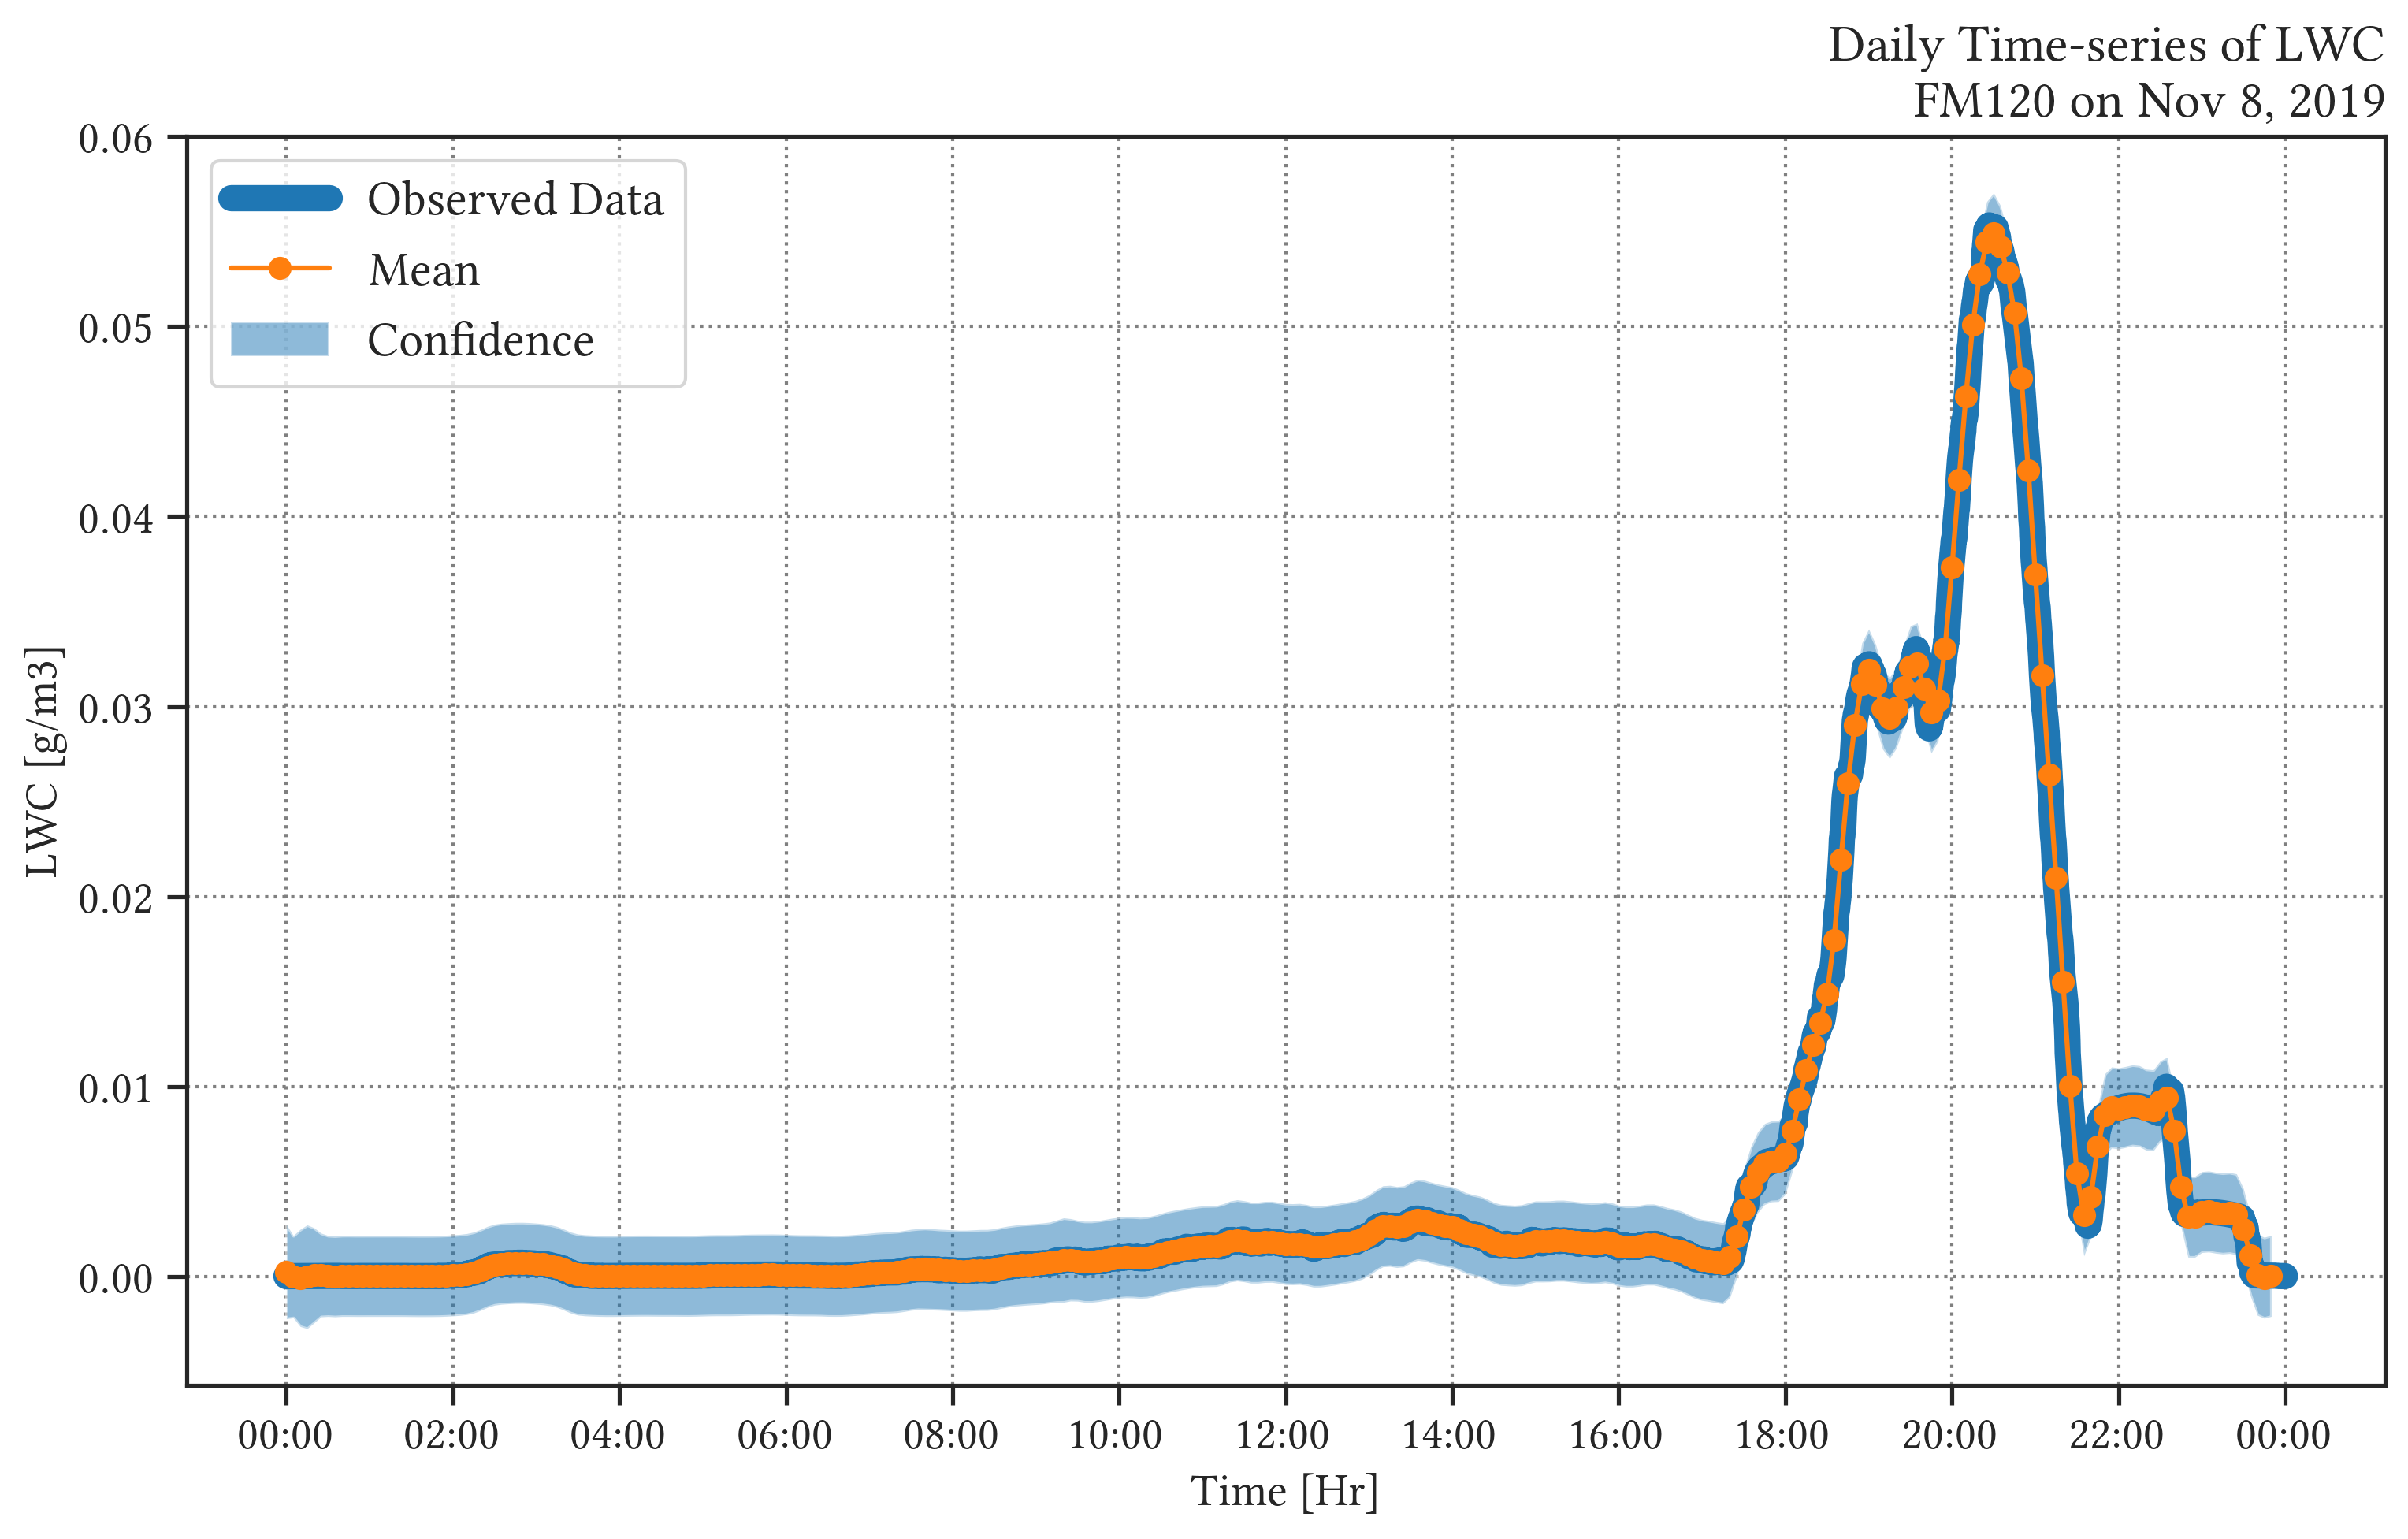
\includegraphics[width=\colwidth]{img/lwc_fm.png}
        \caption{ The time-series of cloud liquid water content (LWC) [g/m$^3$] measured by FM120 \cite{karl2020ro,koik2019ye} on November 8th, 2019, at the Zeppelin Observatory near Ny-\r{A}lesund, Svalbard. Blue dots represent smooth GP posterior (\emph{cf.} Figure \ref{fig:02}), and the orange dots have been sampled from the posterior at a 10-minute interval. The shaded region denotes the 95\% confidence region for the GP posterior distribution. }
        \label{fig:04}
    \end{figure}
  \end{block}

  \begin{block}{Remarks}
    We have introduced a statistical method to analyze noisy time-series observations of low-altitude cloud properties from the cloud particle spectrometer (CDP2) and fog monitor (FM120 \cite{karl2020ro,koik2019ye}). The preliminary analysis shows that the two probes correspond well to each other, although FM120 tends to generally underestimate the values of LWC compared to those from CDP2.

    A more quantitative analysis, especially over the longer term, needs to be performed in order to precisely determine the correlation between the observations from the two probes. Still, we have shown that the high-resolution observations taken from CDP2 can precisely determine the evolution of cloud particles in the low-altitude arctic atmosphere.
  \end{block}

  \begin{block}{References}
    \nocite{*}
    \footnotesize{\bibliographystyle{abbrv}\bibliography{poster}}
  \end{block}

\end{column}

\separatorcolumn
\end{columns}
\end{frame}

\end{document}